% !TEX root = ../thesis.tex

\chapter{Implementierung}
\label{ch:implementierung}

Nachdem nun die theoretischen Grundlagen gelegt sind, wird im Folgenden die Implementierung der Pipeline erklärt.
Zunächst wird in \ref{sec:aufbau} der Aufbau des Programms beschrieben.
Die Interaktion und Parametrisierung wird in \ref{sec:interaktion} erläutert.
In \ref{sec:pipeline} wird dann der gesamte Ablauf der Pipeline und das Zusammenspiel der verschiedenen Komponenten noch einmal zusammengefasst.



\section{Aufbau}
\label{sec:aufbau}

Die Pipeline ist in C++ auf Basis der \ac{PCL} \cite{rusu2011pcl} geschrieben.
Dabei handelt es sich um eine Open-Source-Bibliothek, welche die Arbeit mit 3D-Punktwolken immens vereinfacht.
Sie bietet Möglichkeiten zur Filterung, Segmentierung, Oberflächenrekonstruktion und Visualisierung von Punktwolken, sowie weitere Module.

Neben den zahlreichen unterstützten Anwendungsgebieten und implementierten Algorithmen bietet die \ac{PCL} den weiteren entscheidenden Vorteil, dass sie direkt zu \ac{ROS} \cite{quigley2009ros} kompatibel ist.
Die Kompatibilität wird durch ROS-Nodelets im Paket \texttt{perception\_pcl} hergestellt, sodass Punktwolken, Meshes oder andere Datenstrukturen direkt zwischen \ac{ROS}-basierten Komponenten versendet werden können.

Um eine modulare Verwendung des Tools zu gewährleisten wurde ein einzelnes \ac{ROS}-Paket erstellt.
Die 3D-Datenverarbeitung findet hauptsächlich auf Basis der \ac{PCL} statt, mit einer Grobregistrierung über \ac{OpenGR}.
Zur 2D-Segmentierung über den Watershed-Algorithmus wird OpenCV verwendet.

Weiterhin werden eine aktuelle Version des Ensenso SDKs und die \ac{ROS}-Serviceheader zu den von Mikado versendeten Nachrichten benötigt.
Mit ihrer Hilfe können die aktuellen 2D-Grauwertbilder ausgelesen und zur Segmentierung verwendet werden.



\section{Interaktion und Parametrisierung}
\label{sec:interaktion}

Die Interaktion zwischen Mikado und dem Rekonstruktionstool findet über \ac{ROS} statt.
Dabei handelt es sich um einen \texttt{ros::Subscriber} auf das von Mikado veröffentlichte Topic \texttt{/point\_cloud}.
Bei Aufnahme einer neuen Punktwolke wird somit das Durchlaufen der Pipeline automatisch angestoßen.

Weiterhin lassen sich über \texttt{rosparam set} und \texttt{rosparam get} Parameter setzen oder auslesen.
Diese werden dann im Programm geparst und -- falls nicht vorhanden -- durch Standardwerte ersetzt.
Dies bietet mehrere Vorteile gegenüber anderen Optionen:

\begin{itemize}
\item Parameter können optional über die Konsole, auf Programmebene oder auch gar nicht gesetzt werden.
\item Das Programm muss nicht für jede Konfiguration neu kompiliert werden und kann bei Laufzeit parametrisiert werden.
\item Die Interaktion mit anderen Programmen ist durch die Verwendung der \ac{ROS}-Schnittstelle erheblich vereinfacht.
\end{itemize}

Auch die Triangulation wird durch einen externen Trigger angestoßen.
Dieser wird als \texttt{rosservice} zur Verfügung gestellt, welcher mit dem Output-Dateipfad aufgerufen wird.
Auch hier ist durch die Verwendung der \ac{ROS}-basierten Schnittstelle eine hohe Flexibilität gegeben.



\section{Pipelineablauf}
\label{sec:pipeline}

Der Ablauf der Pipeline ist stark abhängig von der durch den Nutzer gewählten Konfiguration.
Diese kann jedoch auch nach Start des Programms noch geändert werden.
Ohne vorherige Wahl eines Modus werden weder Segmentierung noch Registrierung vorgenommen.

\begin{figure}[H]
    \centering
	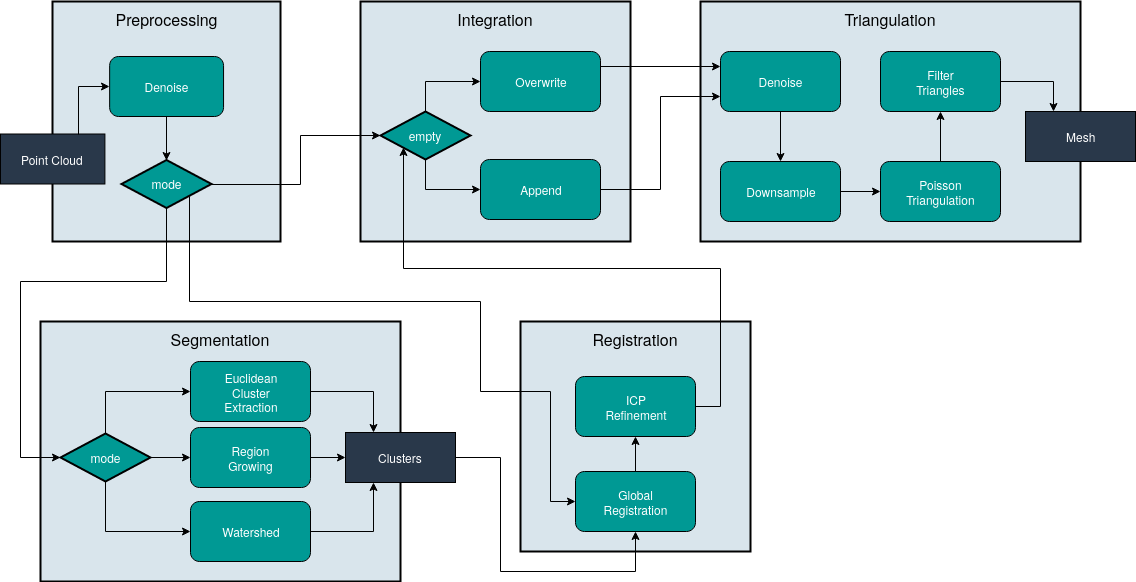
\includegraphics[width=\textwidth]{images/pipeline.png}
	\caption{Ablauf der Pipeline}
	\label{fig:pipeline}
\end{figure}

Der gesamte Ablauf des Prozesses vom Empfang einer Punktwolke bis zur Ausgabe des rekonstruierten Meshs ist in \autoref{fig:pipeline} sichtbar.
Der Programmablauf kann in mehrere verschiedene Blöcke unterteilt werden, welche im Folgenden erläutert werden.


\subsection{Preprocessing}
\label{subsec:pipeline-preprocessing}

Das Preprocessing findet unabhängig von der Wahl des Modus statt.
Nach Empfang einer Punktwolke wird diese zunächst durch ein \texttt{pcl::StatisticalOutlierRemoval} gefiltert.
Das Ziel ist die Eliminierung von unvermeidbarem Sensorrauschen.

In diesem Schritt könnten auch noch andere Preprocessingmethoden durchgeführt werden.
Dabei kann es sich sowohl um ein Downsampling zur Datenreduktion handeln als auch um Prozesse wie eine Normalenschätzung, falls diese nicht bereits vorher stattgefunden hat.


\subsection{Segmentierung}
\label{subsec:pipeline-segmentierung}

Dieser Block wird nur ausgeführt, wenn der entsprechende Modus gewählt ist.
In diesem Schritt findet die Segmentierung der Punktwolke statt.
Je nach gewählter Methode lässt sich dabei zwischen \ac{ECE}, \ac{RG} und Watershed-Segmentierung wählen.
Die Punktwolke wird dabei in einen Vektor gespalten, der die einzelnen Cluster beinhaltet.


\subsection{Registrierung}
\label{subsec:pipeline-registrierung}

Hier wird die Eingabepunktwolke an der bereits integrierten Punktwolke registriert.
Dabei wird zunächst eine globale Schätzung mithilfe von \ac{4PCS} durchgeführt.
Diese Registrierung wird anschließend durch \ac{ICP} verfeinert.

Der Registrierungsprozess wird abgebrochen, falls einer der beiden Registrierungen nicht konvergiert.
Weiterhin kann ein Grenzwert gewählt werden, unter dem der Score liegen muss.
Bei \ac{ICP} beschreibt dieser Score den \ac{MSE}.

Die Registrierung wird durch Parametrisierung aktiviert bzw. deaktiviert.
Hat zuvor eine Segmentierung stattgefunden, wird jeder Cluster seperat diesem Block zugeführt.


\subsection{Integration}
\label{subsec:pipeline-integration}

Dieser Schritt beschreibt das Zusammenführen der beiden Punktwolken.
Es wird vorausgesetzt, dass vorher bereits eine Registrierung stattgefunden hat.

In der Praxis ist dieser Block sehr einfach gehalten.
Liegt die Zahl der Punkte unter einem Grenzwert, werden diese überschrieben.
Ist dies nicht der Fall, müssen die beiden Vektoren konkateniert werden.


\subsection{Triangulierung}
\label{subsec:pipeline-triangulierung}

Entspricht die zusammengeführte Punktwolke den Erwartungen des Nutzers, kann dieser nun die Triangulierung anstoßen.
Dies bedeutet, dass dieser Block nicht automatisch ausgeführt wird.
Der Grund dafür ist, dass es sich um einen sehr zeit-, speicher- und rechenintensiven Vorgang handelt.

Zunächst findet eine weitere Filterung statt.
Dies ermöglicht selbst dann ein brauchbares Ergebnis, falls im Registrierungsschritt keine fehlerfreie Ausrichtung erreicht worden ist.
Im Optimalfall werden die fehlerhaften Daten aufgrund der hohen Punktdichte an der Oberfläche somit größtenteils entfernt.

Nach dem anschließenden Downsampling findet eine Poisson-Triangulierung statt.
Da die Poisson-Triangulierung immer wasserdichte Polygone erzeugt, können hierbei auch inkorrekte Dreiecke generiert werden.
Im letzten Schritt werden daher nun Dreiecke aus dem Polygonnetz entfernt, die eine festgelegte Distanz von der Punktwolke überschreiten.
